
% Begin with describing virtual circuit switching
\begin{section}{Virtual Circuit Switching}

Virtual Circuit Switching is a packet switching methodology in which a dedicated path is established between the source and destination before the actual data transfer begins. All packets on a Virtual-Circuit Switched network are routed using link-specific labels called Virtual Circuit IDs (VCIDs). During the path setup, these forwarding tables are setup in each of the intermediate routers using these VCIDs. When the data transfer is deemed complete, the virtual circuit is torn down, and the forwarding table entries along the path are invalidated.

\end{section}


\begin{section}{Experiment}

    To compare the probability of blocking of a connection in a virtual circuit switched network in two different topologies under different traffic loads, constraints (pessimistic and optimistic), and routing metrics.

\end{section}

\begin{section}{Variables of the Experiment}

    \begin{subsection}{Topology}
        Two topologies are considered for the experiment:
        \begin{enumerate}
            \item NSFNET Topology : A network with 12 nodes and 15 links.
            \item ARPANET Topology : A network with 20 nodes and 32 links.
        \end{enumerate}
    \end{subsection}

    \begin{subsection}{Connections}
    Two types of connections are possible:
    \begin{enumerate}
        \item Connections between any two nodes chosen uniformly at random. In this case the connections can be denied for two reasons:
        \begin{enumerate}
            \item There is no path between the two nodes.
            \item There is insufficient bandwidth available on the path between the two nodes.
        \end{enumerate}
        \item Connections are chosen randomly from the set of reachable pairs of nodes. In this case the connections can be denied only if bandwidth is insufficient.
    \end{enumerate}
    Since we are only interested in the probability of blocking and not the restrictions of the topology, we will consider the second type of connections.
    \end{subsection}

    \begin{subsection}{Traffic Load}
        \begin{enumerate}
            \item Constant traffic load at 64 kbps. This specific value is chosen because voice calls are typically 64 kbps.
            \item Bursty traffic of $(\text{min}, \text{avg}, \text{max}) = (1, x, 10x)$ kbps. The value of $x$ is varied from 2 to 20 with steps of 2.
        \end{enumerate}
    \end{subsection}
    

    \begin{subsection}{Constraints}
        Two types of constraints are considered for the experiment:
        \begin{enumerate}
            \item \textit{Pessimistic constraints}: Assumes each connection uses its maximum bandwidth.
            \item \textit{Optimistic constraints}: Assumes each connections uses bandwidth equal to \\ $\min\left(B_{max},\ B_{avg} + 0.35 \cdot (B_{max} - B_{min}) \right)$
        \end{enumerate}
    \end{subsection}

    \begin{subsection}{Routing Algorithm}
        Two types of routing metrics are considered for computing the shortest and second shortest path: (1) Hop count and (2) Propagation Delay.
    \end{subsection}

\end{section}

\begin{section}{Results}

It was observed that the blocking probability is the same for both the routing metrics, Hop count and Propagation Delay. The following plots and observations hold for both these metrics. \\

\begin{figure}[H]
    \centering
    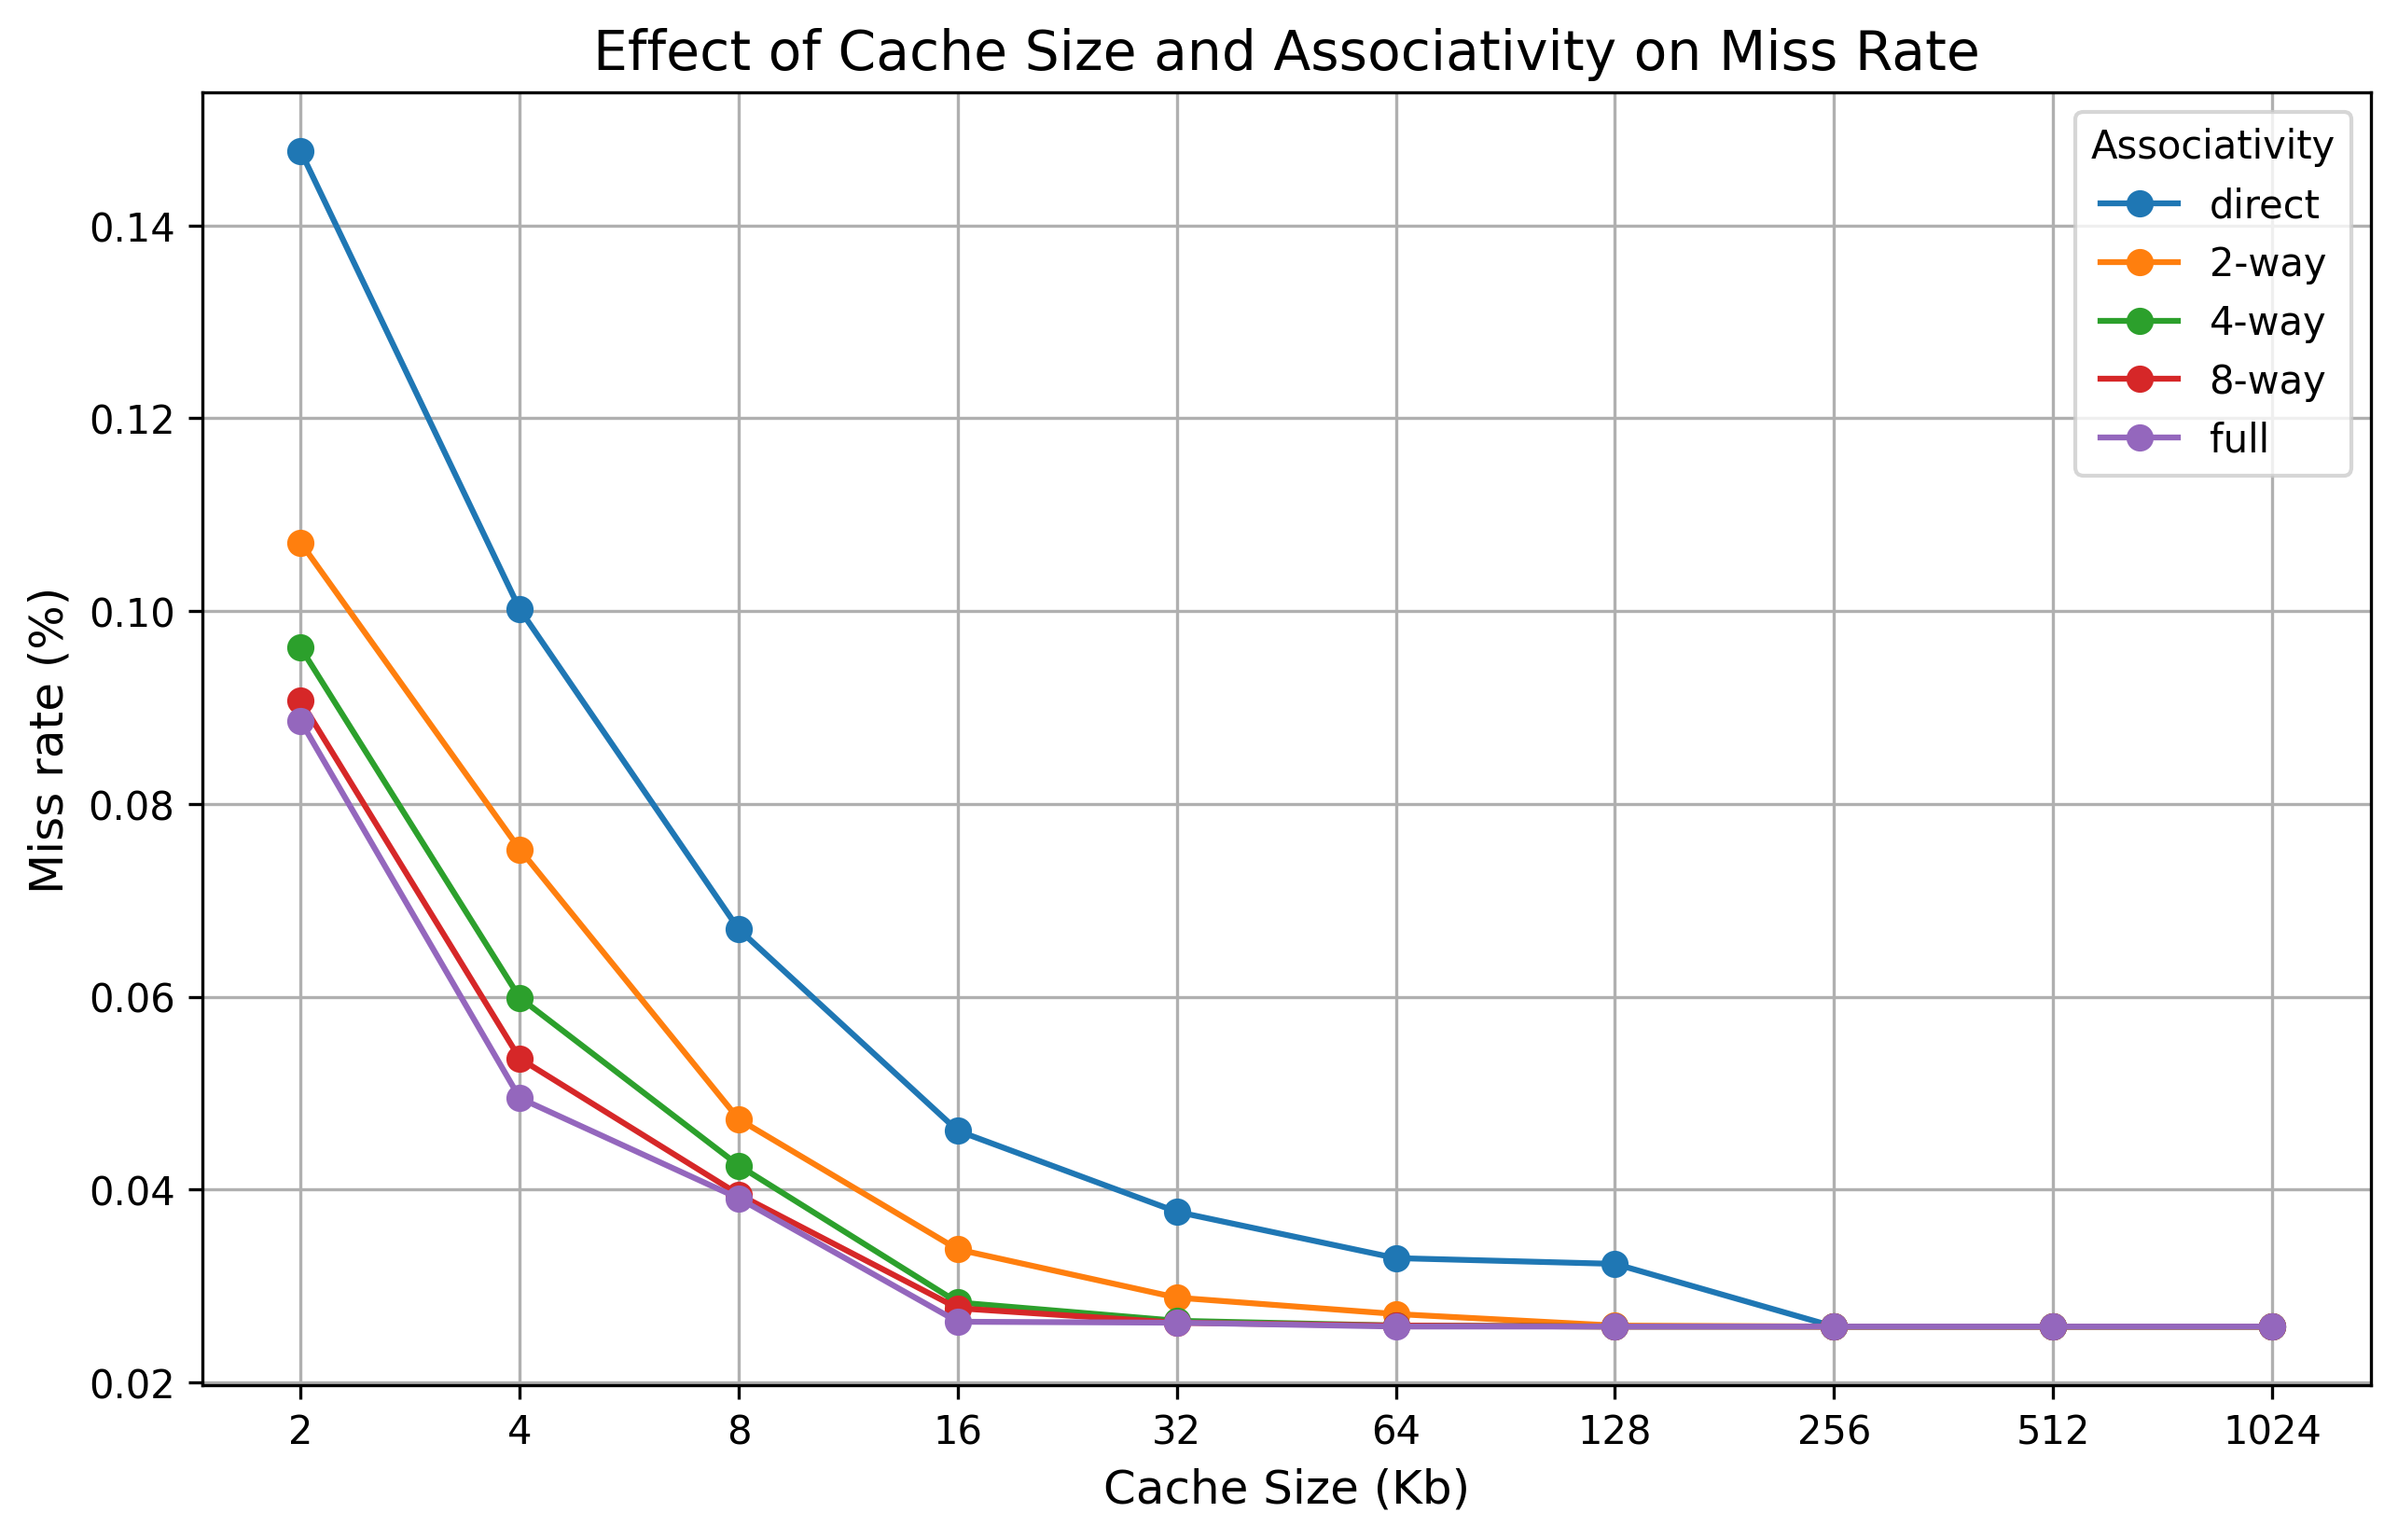
\includegraphics[width=0.8\textwidth]{figures/fig1/fig1.png}
    \caption{Blocking Probability with Constant 64kbps Traffic Load \protect\footnotemark}
    \label{fig:fig1}
\end{figure}
\footnotetext{Since the traffic is constant, both optimistic and pessimistic constraints give the same results.}

As is expected, we see that the blocking probability increases as the number of connections increase. This is because the links start getting saturated and available bandwidth becomes insufficient. \\
Also, since the ARPANET topology has more nodes and links than NSFNET, the number of connections needed to saturate most of the links in ARPANET is higher than that for NSFNET. Thus, we see that for the same number of connections, ARPANET has a lower blocking probability. \\ 


\pagebreak

% make a figure with two subfigures side by side
\begin{figure}[H]
    \centering
    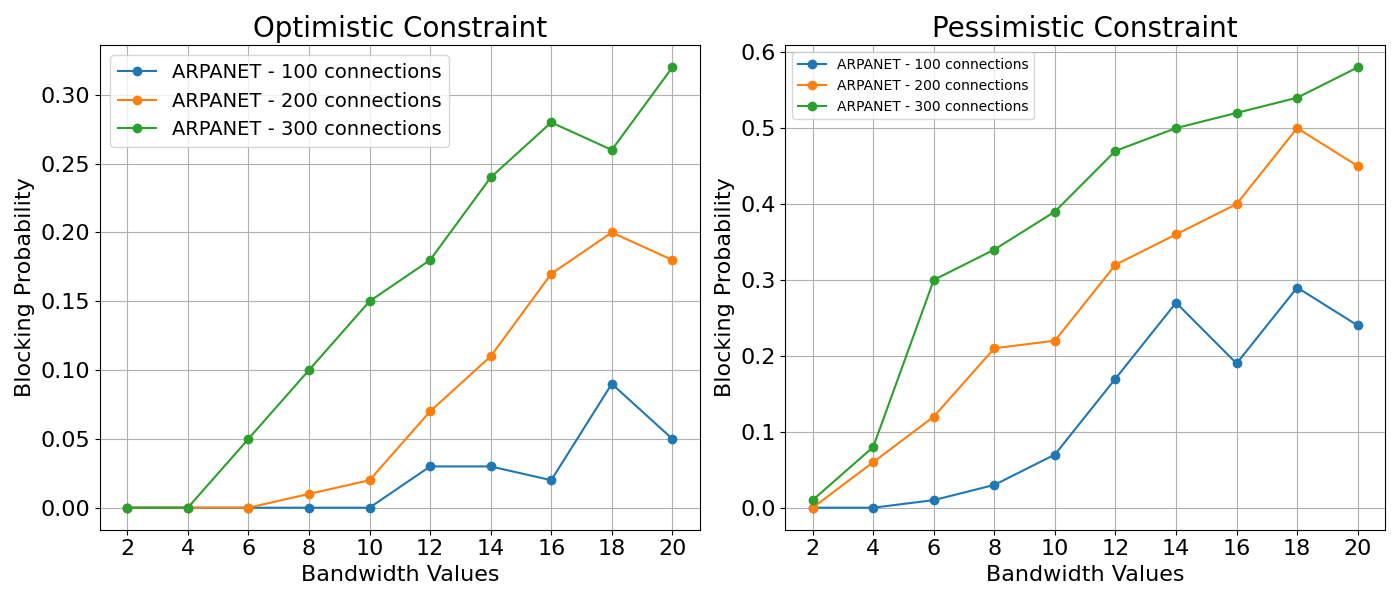
\includegraphics[width=\textwidth]{figures/fig2/fig2a.png}
    \caption{Blocking Probability with Bursty Traffic Load for ARPANET}
    \label{fig:fig2a}
\end{figure}


% make a figure with two subfigures side by side
\begin{figure}[H]
    \centering
    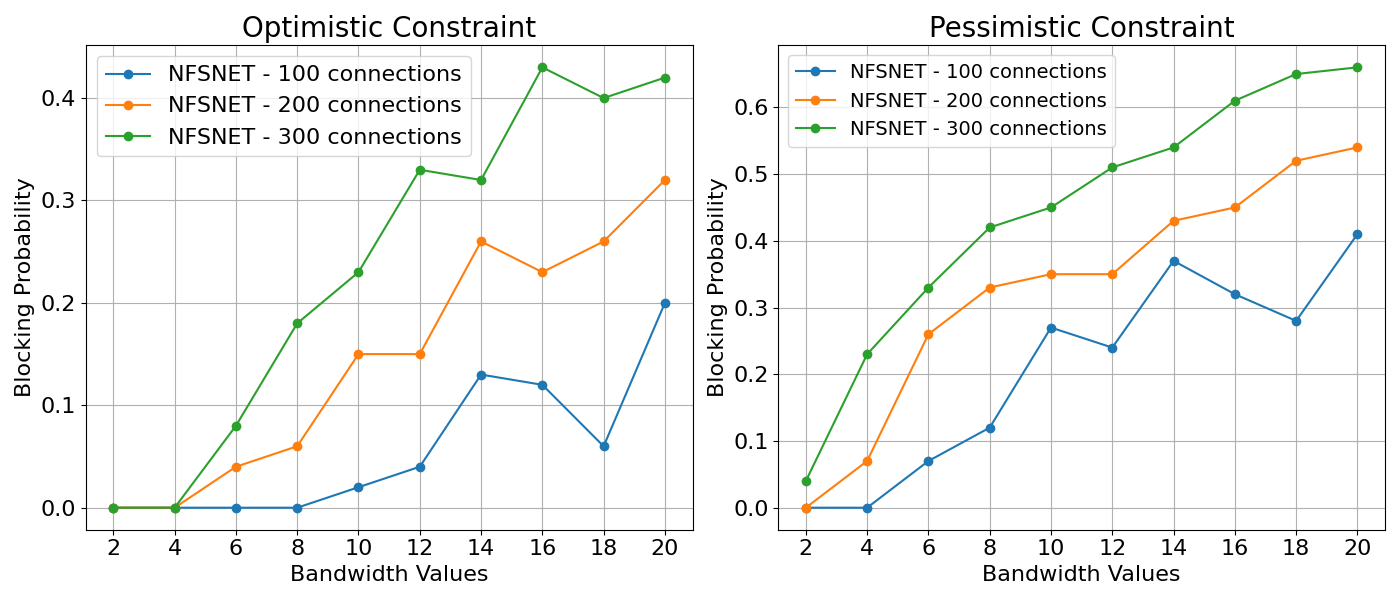
\includegraphics[width=\textwidth]{figures/fig2/fig2b.png}
    \caption{Blocking Probability with Bursty Traffic Load for NSFNET}
    \label{fig:fig2b}
\end{figure}

The blocking probabilities of the two topologies are shown in Figures \ref{fig:fig2a} and \ref{fig:fig2b}. We see that the blocking probability increases as the traffic load increases. Further the increase is more profound in the case of pessimistic constraint as it assumes that the whole bandwidth is consumed by the connection, whereas the optimistic constraint uses a better estimate. \\ \\
Also, as discussed before, the blocking probabilities are higher for more number of connections as the connections compete for the same links in the topology. Further the blocking probability is higher for NSFNET than ARPANET for the same number of connections as ARPANET has more nodes and links. \\ 

\end{section}
